\documentclass{statsoc}
\usepackage{amsmath, amssymb}
\usepackage{graphicx,psfrag,epsf}
\usepackage{enumerate}
\usepackage{natbib}
\usepackage{url} % not crucial - just used below for the URL 

% DON'T change margins - should be 1 inch all around.
\addtolength{\oddsidemargin}{-.5in}%
\addtolength{\evensidemargin}{-.5in}%
\addtolength{\textwidth}{1in}%
\addtolength{\textheight}{-.3in}%
\addtolength{\topmargin}{-.8in}%

%%%% Packages and definitions
\usepackage{xr}
\externaldocument{hillclimbing_statsoc_appendix}

\usepackage[top=0.85in,left=1.0in,right=1.0in,footskip=0.75in]{geometry}

% Use adjustwidth environment to exceed column width (see example table in text)
\usepackage{changepage}

% Use Unicode characters when possible
\usepackage[utf8]{inputenc}

% textcomp package and marvosym package for additional characters
\usepackage{textcomp,marvosym}

\usepackage[ruled]{algorithm}
\usepackage{algorithmic}

% cite package, to clean up citations in the main text. Do not remove.
\usepackage{cite}

% Use nameref to cite supporting information files (see Supporting Information section for more info)
\usepackage{nameref,hyperref}

%\usepackage{amsthm}

% ligatures disabled
\usepackage{microtype}
\DisableLigatures[f]{encoding = *, family = * }

% subcaptions
%\usepackage{subcaption}

% for the beautiful checkmarks
\usepackage{pifont}

\newtheorem{theorem}{Theorem}
\newtheorem{corollary}{Corollary}
\newtheorem{lemma}{Lemma}
\newtheorem{definition}{Definition}
\newtheorem{condition}{Condition}

\DeclareMathOperator*{\argmin}{arg\,min}

%%%%%%%%%%%%%%%%%%%%%%%%%%%%%%%%%%%%%%%%%%%%%%%%%%%%%%%%%%%%%%%%%%%%%%%%%%%%%%%%%%

\title[Tuning Parameter Selection]{Tuning Parameter Selection based on Validation-Error Descent}
\author[Feng and Simon]{Jean Feng}
\address{Department of Biostatistics, University of Washington, Seattle, USA.}
\email{jeanfeng@uw.edu}
\author[Feng and Simon]{Noah Simon}
\address{Department of Biostatistics, University of Washington, Seattle, USA.}
\email{noahsimon@uw.edu}

\begin{document}

\begin{abstract}
In high-dimensional and/or non-parametric regression problems, regularization (or penalization) is used to control model complexity and induce desired structure. Each penalty has a weight parameter that indicates how strongly the structure corresponding to that penalty should be enforced. To date, for problems with $k=2$ or more penalties, tuning these penalty parameters is a challenge. The current gold-standard of calculating validation error over a $k$-dimensional grid of parameter values quickly becomes computationally intractable as $k$ increases. We propose tuning parameters by solving a continuous optimization problem over a validation set and updating the values using a descent-based approach. We show that our method is significantly more efficient than calculating validation error over an entire grid, and empirically achieves the same performance (on scenarios where a grid search could be performed). This descent-based approach enables us to test regularization problems with many penalty parameters, through which we discover new regularization methods with superior accuracy. We also include simulated experiments, and a data analysis, which illustrate the strength of this new method.
\end{abstract}

\keywords{regularization, high-dimensional regression, cross-validation, optimization}

\section{Introduction}
Consider the usual regression framework with $p$ features, $\boldsymbol x_i = (x_{i1},\ldots,x_{ip})^\top$, and a response $y_i$ measured on each of $i=1,\ldots,n$ observations. Let $\boldsymbol X$ denote the $n \times p$ design matrix and $\boldsymbol y$ the response vector. Our goal here is to characterize the conditional relationship between $\boldsymbol y$ and $\boldsymbol X$. In simple low-dimensional problems this is often done by constructing an $f$ in some pre-specified class $\mathcal{F}$ that minimizes a measure of discrepancy between $\boldsymbol y$ and $f(\boldsymbol X)$. Generally, this discrepancy is quantified with some pre-specified loss, $L$. Often $\mathcal{F}$ will endow $f$ with some simple form (e.g. a linear function). For ill-posed or high-dimensional problems ($p \gg n$), there can often be an infinite number of solutions that minimize the loss function $L$ but have high generalization error. A common solution is to use regularization, or penalization, to select models with desirable properties, such as smoothness and sparsity.

In recent years, there has been much interest in combining regularization methods to produce models with multiple desired characteristics. Examples include the elastic net \citep{zou2003regression}, which combines the lasso and ridge penalties, and the sparse group lasso \citep{simon2013sparse}, which combines the group lasso and lasso penalties. The general form of these regression problems is:
\begin{equation} \label {eq:basic}
\hat f(\boldsymbol{\lambda}) = \argmin_{f\in\mathcal{F}} L\left (\boldsymbol{y}, f (\boldsymbol{X}) \right ) + \sum\limits_{i=1}^J \lambda_i P_i(f)
\end{equation}
where $\{P_i\}_{i=1, ..., J}$ are the penalty functions and $\boldsymbol{\lambda} = (\lambda_1, \ldots, \lambda_J)^\top$ are the regularization parameters.

Regularization parameters control the degree of various facets of model complexity, such as the amount of sparsity or smoothness. Often, the goal is to set the parameters to minimize the fitted model's generalization error. One usually estimates this using a training/validation approach (or cross validation). There one fits a model on a training set $(\boldsymbol X_T, \boldsymbol y_T)$ and measures the model's error on a validation set $(\boldsymbol X_V, \boldsymbol y_V)$. The goal then is to choose penalty parameters $\boldsymbol{\lambda}$ that minimize the validation error, as formulated in the following optimization problem:
\begin{equation}
\begin{array}{c}
\min_{\boldsymbol{\lambda} \in \Lambda} L\left (\boldsymbol{y}_V, \hat f (\boldsymbol{X}_V | \boldsymbol{\lambda}) \right) \\
\text{s.t. } \hat f(\cdot | \boldsymbol{\lambda}) = \argmin_{f\in\mathcal{F}} L \left (\boldsymbol{y}_T, f (\boldsymbol{X}_T) \right) + \sum\limits_{i=1}^J \lambda_i P_i(f)
\end{array}
\label{jointopt}
\end{equation}
Here $\Lambda$ is some set that $\boldsymbol{\lambda}$ are known to be in, which is often just $\mathbb{R}^{J}_+$.

The simplest approach to solving \eqref{jointopt} is brute force: one fits models over a grid of parameter values and selects the model with the lowest validation error. As long as the grid is large and fine enough, this method of ``grid search" will find a solution close to the global optimum. This approach is the current standard for choosing penalty parameters via training/validation. Unfortunately, it is computationally intractable in cases with more than two parameters since the runtime is exponential in the number of parameters. For certain special cases, there are more efficient ways of tuning the parameters \citep{golub1979generalized}, \citep{wood2000modelling}, but there is no general solution to date.

In this paper, we propose leveraging the tools of optimization to solve \eqref{jointopt}. We give a gradient descent algorithm for minimizing the validation error over the penalty parameter space. In contrast to an exhaustive ``grid search'', this ``descent-based'' optimization makes use of the smoothness of our validation-error surface. \eqref{jointopt} is generally not convex and thus we may not find the global minimum with a simple descent-based approach. However, in practice we find that simple descent gives competitive solutions.

In simulation studies we show that our descent-based optimization produces solutions with the same validation error as those from grid search. In addition, we find that our approach is highly efficient and can solve regressions with hundreds of penalty parameters. Finally, we use this method to analyze regularization methods that were previously computationally intractable. Through this, we discover that a variant of sparse group lasso with many more penalty parameters can significantly decrease error and produce more meaningful models.

\citet{lorbert2010descent} presented some related work on this topic. They solved linear regression problems by updating regression coefficients and regularization parameters using cyclical coordinate gradient descent. We take a more general approach that allows us to apply this descent-based optimization to a wide array of problems. We present examples in this paper that demonstrate the wide applicability of our method.

In Section~\ref{defineDescJointOpt}, we describe descent-based optimization in detail and present an algorithm for solving it in example regressions. In Section~\ref{results1}, we show that our method achieves validation errors as low as those achieved by grid search. In Section~\ref{results1}, we explore variants of the example regression problems that have many more regularization parameters and demonstrate that solving \eqref{jointopt} is still computationally tractable. Finally, we present results on data predicting colitis status from gene expression in Section~\ref{realDataResults}.

\section{Descent-based Joint Optimization}\label{defineDescJointOpt}
\subsection{Definition}
In this manuscript we will restrict ourselves to classes $\mathcal{F} = \left\{f_{\boldsymbol \theta}\middle| \boldsymbol \theta\in\Theta\right\}$, which, for a fixed sample size $n$, are in some finite dimensional space $\Theta$. This is not a large restriction: the class of linear functions functions meets this requirement; as does any class of finite dimensional parametric functions. Even non-parametric methods generally either use a growing basis expansion (e.g. Polynomial regression, smoothing-splines, wavelet-based-regression, locally-adaptive regression splines \citep{tsybakov2008introduction}, \citep{wahba1981spline}, \citep{donoho1994ideal}, \citep{mammen1997locally}), or only evaluate the function at the observed data-points (eg. trend filtering, fused lasso, \citep{kim2009ell_1}, \citep{tibshirani2005sparsity}). In these non-parametric problems, for any fixed $n$, $\mathcal{F}$ is representable as a finite dimensional class.
We can therefore rewrite \eqref{eq:basic} in the following form:
\begin{equation}\label{eq:train_disc}
\argmin_{\boldsymbol \theta \in \Theta} L(\boldsymbol{y}, f_{\boldsymbol \theta}(\boldsymbol{X})) + \sum\limits_{i=1}^J \lambda_i P_i(\boldsymbol \theta)
\end{equation}

Suppose that we use a training/validation split to select penalty parameters $\boldsymbol{\lambda} = (\lambda_1, ..., \lambda_J)^\top$. Let the data be partitioned into a training set $(\boldsymbol{y}_T , \boldsymbol{X}_T)$ and validation set $(\boldsymbol{y}_V, \boldsymbol{X}_V)$. We can rewrite the joint optimization problem \eqref{jointopt} over this finite-dimensional class as:
\begin{equation}
\begin{array}{c}
\argmin_{\boldsymbol{\lambda} \in \Lambda} L(\boldsymbol{y}_V, f_{\hat{\boldsymbol \theta}(\boldsymbol{\lambda})}(\boldsymbol{X}_V)) \\
\text{s.t. } {\hat{\boldsymbol \theta}(\boldsymbol{\lambda})} = \argmin_{\boldsymbol \theta \in \Theta} L(\boldsymbol{y}_T, f_{\boldsymbol \theta} (\boldsymbol{X}_T)) + \sum\limits_{i=1}^J \lambda_i P_i(\boldsymbol \theta)
\end{array}
\label{jointopt2}
\end{equation}
For the remainder of the manuscript we will assume that \eqref{eq:train_disc} for the training set is strictly convex in $\boldsymbol \theta$. This ensures that there is a unique $\hat{\boldsymbol \theta}(\boldsymbol{\lambda})$ which perturbs continuously in $\boldsymbol{\lambda}$.

\eqref{jointopt2} is the explicit, though often unstated, criterion that training/validation methods attempt to minimize when choosing penalty parameters. The current standard is to minimize this using an exhaustive grid search. Grid-based methods solve the joint optimization problem by fitting models over a $J$-dimensional grid in the penalty parameter space; so the computational runtime grows exponentially with the number of penalty parameters. While the approach is simple and powerful for a single penalty parameter, optimizing even moderate-dimensional functions (3+) via exhaustive grid search is inefficient (and quickly becomes completely intractable).  In addition, \eqref{jointopt2} is generally a continuous, piecewise-smooth problem. An exhaustive search ignores information available from the smoothness of the surface.

We propose solving \eqref{jointopt2} by using the tools of smooth optimization. In particular we discuss iterative methods, based on walking in a descent direction until convergence to a local minimum. In the simple case where the criterion is differentiable with respect to the penalty parameters, it is straightforward to use gradient descent or some variant thereof. We show that, with some slight tweaks, gradient descent can be also applied in situations where the penalty is only differentiable in certain directions.

Figure \ref{fig:compare} illustrates the difference between these two approaches. Grid search fits a model at every grid point, many of which are not close to the global (or local) minima. In contrast, descent-based methods incorporate information about the shape of the local neighborhood to choose an intelligent descent direction. It explores the space more efficiently since it avoids penalty parameter values unlikely to yield good models.

\begin{figure}
\centering
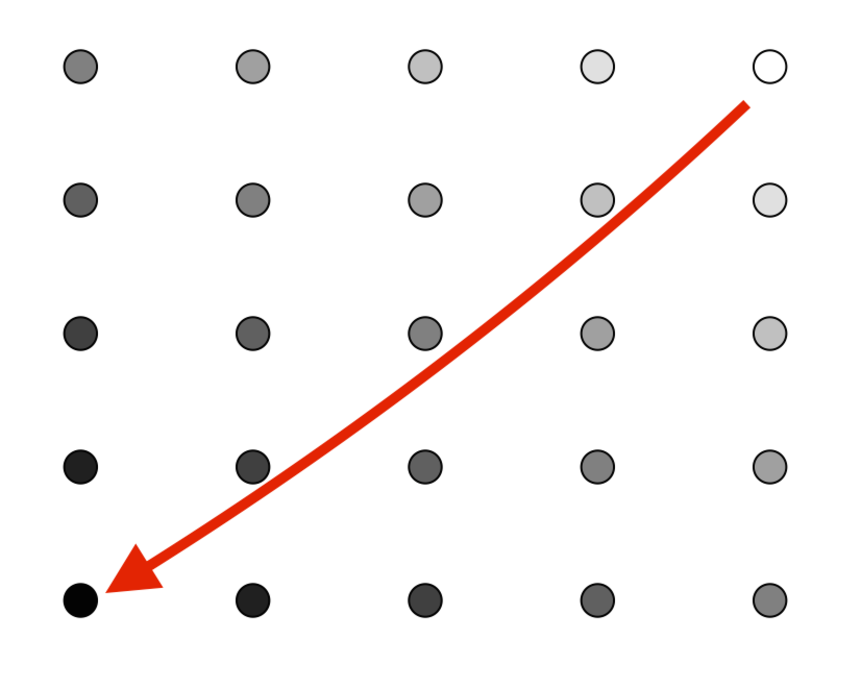
\includegraphics[height=30mm]{grid_search_vs_descent.pdf}
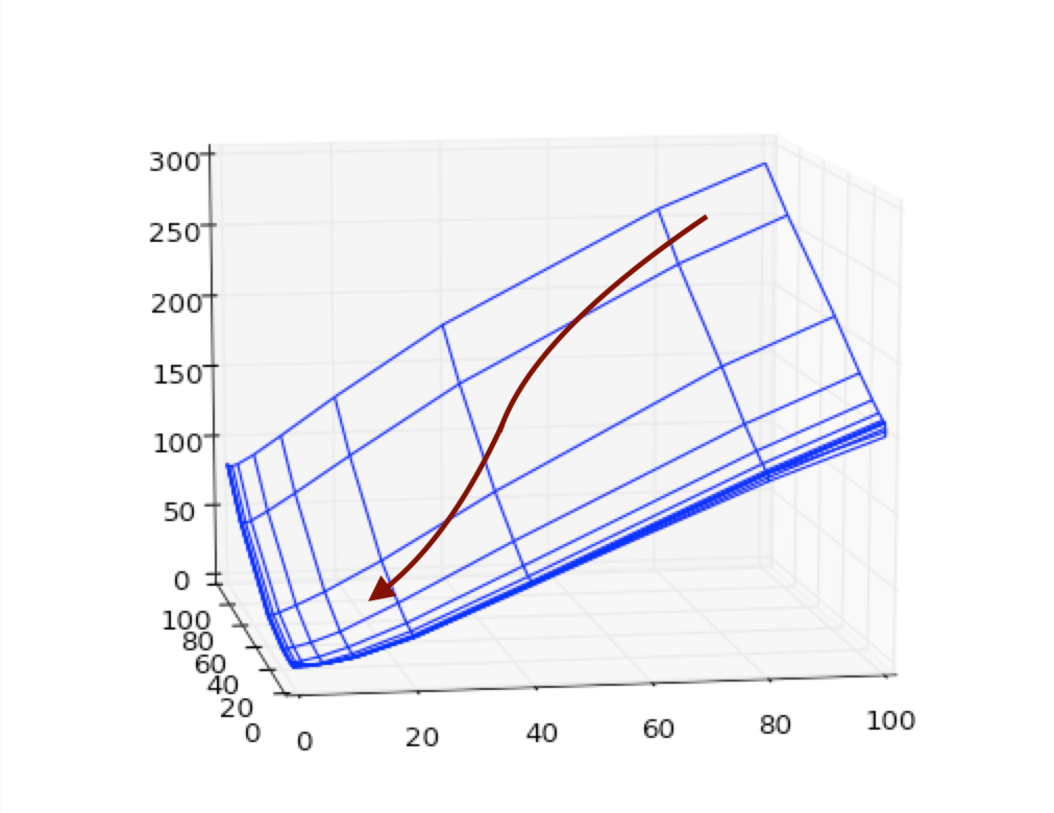
\includegraphics[height=35mm]{surface_in_regularization_parameters.pdf}
\caption{Left: A hypothetical grid of $(\lambda_1,\lambda_2)$ points that an exhaustive grid search would fit models for. The darkness of each point indicates the validation cost; dark points mean lower cost. In this example, descent-based optimization would takes steps along the arrow, while a grid search would have to consider all grid points, many of which are obviously poor candidates. Right: The same example with validation loss now on the vertical axis.}
\label{fig:compare}
\end{figure}

To ease exposition, we will assume throughout the remainder of the manuscript that $L \left( \boldsymbol{y}_V, f_{\boldsymbol \theta}(\boldsymbol{X}_V) \right)$ is differentiable in $\boldsymbol \theta$. This assumption is met if both 1) $f_{\boldsymbol \theta}(\boldsymbol{X}_V)$ is continuous as a function of $\boldsymbol \theta$; and 2) $L\left(\boldsymbol{y}_V,\cdot\right)$ is smooth. Examples include the squared-error, logistic, and poisson loss functions, though not the hinge loss.

\subsection{Smooth Training Criterion}
Let us denote the training criterion as follows
\begin{equation}
L_T\left(\boldsymbol \theta, \boldsymbol{\lambda}\right) \equiv L(\boldsymbol{y}_T, f_{\boldsymbol \theta} (\boldsymbol{X}_T)) + \sum\limits_{i=1}^J \lambda_i P_i(\boldsymbol \theta)
\label{train}
\end{equation}
First we consider the simple case where $L_T\left(\boldsymbol \theta, \boldsymbol{\lambda}\right)$ is smooth as a function of $(\boldsymbol \theta, \boldsymbol{\lambda})$. In this case, the validation loss is differentiable as a function of $\boldsymbol{\lambda}$. So we can directly apply gradient descent to solve~\eqref{jointopt2}, as described in Algorithm~\ref{alg:basic}.

\begin{algorithm}
\caption{\label{alg:basic} Gradient Descent for Smooth Training Criterions}
\begin{algorithmic}
        \STATE{Initialize $\boldsymbol{\lambda}^{(0)}$.}
        \FOR{each iteration $k=0,1,...$ until stopping criteria is reached}
        \STATE{Perform gradient step with step size $t^{(k)}$
	\begin{equation}
	\boldsymbol{\lambda}^{(k+1)} := \boldsymbol{\lambda}^{(k)} -
	\left . t^{(k)} 
	\nabla_{\boldsymbol{\lambda}} L \left( \boldsymbol{y}_V, f_{\hat{\boldsymbol \theta}(\boldsymbol{\lambda})}(\boldsymbol{X}_V)  \right )
	\right |_{\boldsymbol{\lambda} = \boldsymbol{\lambda}^{(k)}}
	\end{equation}
	}
	\ENDFOR
\end{algorithmic}
\end{algorithm}
There are a number of potential ways to choose the step-size $t^{(k)}$. Choice of step-size is discussed further in Section~\ref{sec:alg_details}.
% --- two simple options are fixed size $t^{(k)} = t$ and harmonically decreasing $t^{(k)} = t/k$.\\
\vspace{1mm}

\noindent
\textbf{Calculating the Gradient}:
The gradient can be found using the chain rule:
\begin{equation}
\nabla_{\boldsymbol{\lambda}} L \left( \boldsymbol{y}_V, f_{\hat{\boldsymbol \theta}(\boldsymbol{\lambda})}(\boldsymbol{X}_V) \right ) = 
\left [
\left . \frac{\partial}{\partial \boldsymbol \theta} L ( \boldsymbol{y}_V, f_{\boldsymbol \theta}(\boldsymbol{X}_V)) \right |_{\boldsymbol \theta=\hat{\boldsymbol \theta}(\boldsymbol \lambda)}
\right ]^\top 
\frac{\partial}{\partial \boldsymbol{\lambda}} \hat{\boldsymbol \theta}(\boldsymbol{\lambda})
\label{chainrule}
\end{equation}
The first term, $\frac{\partial}{\partial \boldsymbol \theta} L ( \boldsymbol{y}_V, f_{\boldsymbol \theta}(\boldsymbol{X}_V))$, is problem specific, but generally straightforward to calculate. To calculate the second term, $\frac{\partial}{\partial \boldsymbol{\lambda}} \hat{\boldsymbol \theta}(\boldsymbol{\lambda})$, we note that $\hat{\boldsymbol \theta}(\boldsymbol{\lambda})$ minimizes \eqref{train}. Since \eqref{train} is smooth,
\begin{equation}
\nabla_\theta 
\left . \left (
L(\boldsymbol{y}_T, f_{\boldsymbol \theta} (\boldsymbol{X}_T)) +
\sum\limits_{i=1}^J \lambda_i P_i(\boldsymbol \theta)
\right ) \right |_{\boldsymbol \theta = \hat {\boldsymbol \theta}(\boldsymbol{\lambda})}
= \boldsymbol{0}.
\label{eq:grad}
\end{equation}
Taking the derivative of both sides of \eqref{eq:grad} in $\boldsymbol{\lambda}$ and solving for $\frac{\partial}{\partial \boldsymbol{\lambda}} \hat{\boldsymbol \theta}(\boldsymbol{\lambda})$, we get:
\begin{equation}
\frac{\partial}{\partial \boldsymbol{\lambda}} \hat{\boldsymbol \theta}(\boldsymbol{\lambda}) = 
- \left . \left [ \left [
 \nabla_\theta^2 \left (  L \left (\boldsymbol{y}_T, f_{\boldsymbol \theta} (\boldsymbol{X}_T) \right)  +  \sum\limits_{i=1}^J \lambda_i P_i(\boldsymbol \theta)  \right )  \right ]^{-1}
\nabla_{\boldsymbol \theta} P(\boldsymbol \theta)
\right ]
\right |_{\boldsymbol \theta = \hat {\boldsymbol \theta}(\boldsymbol{\lambda})}
\label{implicitDifferentiation}
\end{equation}
where $\nabla_{\boldsymbol \theta} P(\boldsymbol \theta)$ is the matrix with columns $\{\nabla_{\boldsymbol \theta} P_i(\boldsymbol \theta)\}_{i=1:J}$.

We can plug \eqref{implicitDifferentiation} into \eqref{chainrule} to get $\nabla_{\boldsymbol{\lambda}} L \left ( \boldsymbol{y}_V, f_{\hat{\boldsymbol \theta}(\boldsymbol{\lambda})}(\boldsymbol{X}_V) \right )$. Note that because $\frac{\partial}{\partial \boldsymbol{\lambda}} \hat{\boldsymbol \theta}(\boldsymbol{\lambda})$ is defined in terms of $\hat{\boldsymbol \theta}\left(\boldsymbol{\lambda}\right)$, each gradient step requires minimizing the training criterion first. The updated version of Algorithm~\ref{alg:basic} with the specific gradient calculations is given in the Appendix.

\subsection{Nonsmooth Training Criterion}
When the penalized training criterion in the joint optimization problem is not smooth, gradient descent cannot be applied. Nonetheless, we find that in many problems, the solution $\hat{\boldsymbol \theta}\left(\boldsymbol{\lambda}\right)$ is smooth at almost every $\boldsymbol{\lambda}$ (eg. Lasso, Group Lasso, Trend Filtering); this means that we can indeed apply gradient descent in practice. In this section, we characterize these problems that are almost everywhere smooth. In addition, we provide a solution for deriving $\frac{\partial}{\partial \boldsymbol{\lambda}} \hat{\boldsymbol \theta}(\boldsymbol{\lambda})$ since calculating the gradient is a challenge in and of itself. This is then incorporated into an algorithm for tuning $\boldsymbol{\lambda}$ using gradient descent.

To characterize problems that are almost everywhere smooth, we begin with three definitions:
\begin{definition}
The differentiable space of a real-valued function $L$ at a point $\boldsymbol \eta$ in its domain is the set of vectors along which the directional derivative of $L$ exists.
\begin{equation}
\Omega^{L}(\boldsymbol \eta) = \left \{ \boldsymbol u \middle | \lim_{\epsilon \rightarrow 0} \frac{L(\boldsymbol \eta + \epsilon \boldsymbol u) - L(\boldsymbol \eta)}{\epsilon} \text{ exists } \right \}
\end{equation}
\end{definition}

\begin{definition}
$S$ is a local optimality space for a convex function $L(\cdot, \boldsymbol \lambda_0)$ if there exists a neighborhood $W$ containing $\boldsymbol \lambda_0$ such that for every $\boldsymbol \lambda \in W$,
\begin{equation}
\argmin_{\boldsymbol \theta \in \Theta} L(\boldsymbol \theta, \boldsymbol \lambda) =
\argmin_{\boldsymbol \theta \in S} L(\boldsymbol \theta, \boldsymbol \lambda)
\end{equation}
\end{definition}

\begin{definition}
Let matrix $\boldsymbol B = [ \boldsymbol b_1 \hdots \boldsymbol b_p ] \in \mathbb{R}^{n \times p}$ have orthonormal columns. Let $f$ be a real-valued function over $\mathbb{R}^n$ and suppose its first and second directional derivatives of $f$ with respect to the columns in $\boldsymbol B$ exist. The Gradient vector and Hessian matrix of $f$ with respect to $\boldsymbol B$ are defined respectively as
\begin{equation}\label{eq:hess}
_{\boldsymbol B} \nabla f  =
\left (
\begin{array}{c}
\frac{\partial f}{\partial \boldsymbol b_1} \\
\frac{\partial f}{\partial \boldsymbol b_2} \\
\vdots\\
\frac{\partial f}{\partial \boldsymbol b_p}\\
\end{array}
\right ) \in \mathbb{R}^p;
\quad
_{\boldsymbol B}\nabla^2 f =
\left (
\begin{array}{cccc}
\frac{\partial^2 f}{\partial b_1^2} & \frac{\partial^2 f}{\partial b_1 \partial b_2} & ...  & \frac{\partial^2 f}{\partial b_1 \partial b_p} \\
\frac{\partial^2 f}{\partial b_2 \partial b_1} & \frac{\partial^2 f}{\partial b_2^2} & ...  & \frac{\partial^2 f}{\partial b_2 \partial b_p} \\
\vdots & \vdots &  \ddots & \vdots \\
\frac{\partial^2 f}{\partial b_p \partial b_1} & \frac{\partial^2 f}{\partial b_p \partial b_2} & ...  & \frac{\partial^2 f}{\partial b_p^2} \\
\end{array}
\right ) \in \mathbb{R}^{p \times p}
\end{equation}
\end{definition}

Using these definitions we can now give three conditions which together are sufficient for the differentiability of $L \left( \boldsymbol{y}_V, f_{\hat{\boldsymbol \theta}(\boldsymbol{\lambda})}(\boldsymbol{X}_V) \right )$ almost everywhere.

\begin{condition}
For almost every $\boldsymbol{\lambda}$, the differentiable space $\Omega^{L_T(\cdot, \boldsymbol{\lambda})}(\hat{\boldsymbol \theta}\left(\boldsymbol{\lambda}\right))$ is a local optimality space for $L_T\left(\cdot,\boldsymbol{\lambda}\right)$.
\end{condition}

\begin{condition}
For almost every $\boldsymbol{\lambda}$, $L_T\left(\cdot, \cdot\right)$ restricted to $\Omega^{L_T(\cdot, \cdot)}(\hat{\boldsymbol \theta}\left(\boldsymbol{\lambda}\right), \boldsymbol{\lambda})$ is twice continuously differentiable within some neighborhood of $\boldsymbol{\lambda}$.
\end{condition}

\begin{condition}
For almost every $\boldsymbol{\lambda}$, there exists an orthonormal basis $\boldsymbol B$ of $\Omega^{L_T(\cdot, \boldsymbol{\lambda})}(\hat{\boldsymbol \theta}\left(\boldsymbol{\lambda}\right))$ such that the Hessian of $L_T\left(\cdot, \boldsymbol{\lambda}\right)$ at $\hat{\boldsymbol \theta}\left(\boldsymbol{\lambda}\right)$ with respect to $\boldsymbol B$ is invertible.

\end{condition}
Note that if condition 3 is satisfied, the Hessian of $L_T \left(\cdot, \boldsymbol{\lambda}\right)$ with respect to any orthonormal basis of $\Omega^{L_T(\cdot, \boldsymbol{\lambda})}(\hat{\boldsymbol \theta}\left(\boldsymbol{\lambda}\right))$ is invertible.

Putting all these conditions together, the following theorem establishes that the gradient exists almost everywhere and provides a recipe for calculating it.

\begin{theorem}
Suppose our optimization problem is of the form in \eqref{jointopt2}, with $L_T\left(\boldsymbol \theta, \boldsymbol{\lambda}\right)$ defined as in \eqref{train}.

Suppose that $L \Big( \boldsymbol{y}_V, f_{\boldsymbol \theta}(\boldsymbol{X}_V)\Big)$ is continuously differentiable in $\boldsymbol \theta$, and conditions $1$, $2$, and $3$, defined above, hold.

Then the validation loss $L(\boldsymbol{y_V}, f_{\hat {\boldsymbol\theta}(\boldsymbol{\lambda})}(\boldsymbol{X_V}))$ is continuously differentiable with respect to $\boldsymbol{\lambda}$ for almost every $\boldsymbol{\lambda}$. Furthermore, the gradient of $L(\boldsymbol{y_V}, f_{\hat \theta(\boldsymbol{\lambda})}(\boldsymbol{X_V}))$, where it is defined, is
\begin{equation}
\nabla_{\boldsymbol{\lambda}} L \left ( \boldsymbol{y_V}, f_{\hat {\boldsymbol \theta}(\boldsymbol{\lambda})}(\boldsymbol{X_V}) \right) =
\left [ \left .
\frac{\partial}{\partial \boldsymbol \theta} L(\boldsymbol{y_V}, f_{\boldsymbol \theta}(\boldsymbol{X_V}))
\right |_{\boldsymbol \theta=\tilde{\boldsymbol \theta}(\boldsymbol \lambda)} \right ]^\top
\frac{\partial}{\partial \boldsymbol{\lambda}} \tilde{\boldsymbol \theta}(\boldsymbol{\lambda})
\end{equation}
where
\begin{equation}
\tilde{\boldsymbol \theta}(\boldsymbol{\lambda}) = \argmin_{\boldsymbol \theta \in \Omega^{L_T(\cdot, \boldsymbol{\lambda})}(\hat {\boldsymbol \theta}(\boldsymbol{\lambda}))} L_T(\boldsymbol \theta , \boldsymbol{\lambda})
\label{restrictedmodelparams}
\end{equation}
\label{thethrm}
\end{theorem}

We can therefore construct a gradient descent procedure based on the model parameter constraint in \eqref{restrictedmodelparams}. At each iteration, let matrix $\boldsymbol U$ have orthonormal columns spanning the differentiable space $\Omega^{L_T(\cdot, \boldsymbol{\lambda})}(\hat {\boldsymbol \theta}(\boldsymbol{\lambda}))$. Since this space is also a local optimality space, it is sufficient to minimize the training criterion over the column space of $\boldsymbol U$. The joint optimization problem can be reformulated using $\boldsymbol U \hat {\boldsymbol \beta}(\boldsymbol{\lambda})$ as the model parameters instead:
\begin{equation}
\begin{array}{c}
\min_{\boldsymbol \lambda \in \Lambda} L(\boldsymbol y_V, f_{\boldsymbol U \hat{\boldsymbol \beta} (\boldsymbol \lambda) }(\boldsymbol X_V)) \\
\text{s.t. } \hat{\boldsymbol \beta} (\boldsymbol \lambda) =
\argmin_{\boldsymbol \beta}
L(\boldsymbol y_T, f_{\boldsymbol U \boldsymbol \beta}(\boldsymbol X_T))
+ \sum\limits_{i=1}^J \lambda_i P_i(\boldsymbol U \boldsymbol \beta)
\end{array}
\end{equation}

This locally equivalent problem now reduces to the simple case where the training criterion is smooth. As mentioned previously, implicit differentiation on the gradient condition then gives us $\frac{\partial}{\partial \boldsymbol \lambda}\hat{\boldsymbol \beta}(\boldsymbol \lambda)$, which gives us the value of interest
\begin{equation}
\frac{\partial}{\partial \boldsymbol \lambda}
\hat{\boldsymbol \theta}(\boldsymbol \lambda) =
\boldsymbol U
\frac{\partial}{\partial \boldsymbol \lambda}\hat{\boldsymbol \beta}(\boldsymbol \lambda)
\end{equation}
Note that because the differentiable space is a local optimality space and is thus locally constant, we can treat $\boldsymbol U$ as a constant in the gradient derivations. Algorithm~\ref{alg:gradDescent} provides the exact steps for tuning the regularization parameters.

\begin{algorithm}
\caption{\label{alg:gradDescent} Joint Optimization with Gradient Descent}
  \begin{algorithmic}
        \STATE{
        		Initialize $\boldsymbol{\lambda}^{(0)}$.
	}
        \FOR { each iteration $k=0,1,...$ until stopping criteria is reached}
		\STATE{
              		Solve for $\hat {\boldsymbol \theta}(\boldsymbol{\lambda}^{(k)}) = \argmin_{\theta \in \Theta} L_T(\boldsymbol \theta, \boldsymbol{\lambda}^{(k)})$.
		}
              	\STATE{
			Construct matrix $\boldsymbol U^{(k)}$, an orthonormal basis of $\Omega^{L_T(\cdot, \boldsymbol{\lambda})}\left (\hat{\boldsymbol \theta}(\boldsymbol{\lambda}^{(k)}) \right )$.
		}
              	\STATE{
			Define the locally equivalent joint optimization problem
                            \begin{equation*}
                            \begin{array}{c}
                            \min_{\boldsymbol \lambda \in \Lambda} L(\boldsymbol y_V, f_{\boldsymbol U^{(k)} \hat{\boldsymbol \beta} (\boldsymbol \lambda) }(\boldsymbol X_V)) \\
                            \text{s.t. } \hat{\boldsymbol \beta} (\boldsymbol \lambda) =
                            \argmin_{\boldsymbol \beta}
                            L(\boldsymbol y_T, f_{\boldsymbol U^{(k)} \boldsymbol \beta}(\boldsymbol X_T))
                            + \sum\limits_{i=1}^J \lambda_i P_i(\boldsymbol U^{(k)} \boldsymbol \beta)
                            \end{array}
                            \end{equation*}
		}              
              	\STATE{
			Calculate $\frac{\partial}{\partial \boldsymbol \lambda} \hat{\boldsymbol \beta}(\boldsymbol{\lambda})|_{\boldsymbol{\lambda} = \boldsymbol{\lambda}^{(k)}}$ where $\frac{\partial}{\partial \boldsymbol \lambda} \hat{\boldsymbol \beta}(\boldsymbol{\lambda})$ is
                               \begin{equation*}
                    		-  \left . \left [
                    		_{\boldsymbol U^{(k)}}\nabla^2 \left (
                    			 L(\boldsymbol{y}_T, f_{\boldsymbol U^{(k)}\boldsymbol \beta} (\boldsymbol{X}_T))  + 
                    			 \sum\limits_{i=1}^J \lambda_i P_i(\boldsymbol U^{(k)}\boldsymbol \beta)
                    		\right )
                    		\right ]^{-1}
                    		_{\boldsymbol U^{(k)}}\nabla P(\boldsymbol U^{(k)}\boldsymbol \beta)
                    		\right |_{\boldsymbol \beta =  \hat{\boldsymbol \beta}(\boldsymbol \lambda)}
                               \end{equation*}
			with $_{\boldsymbol U^{(k)}}\nabla^2$ and $_{\boldsymbol U^{(k)}}\nabla$ are as defined in \eqref{eq:hess}.
		}
              
              	\STATE{
			Calculate the gradient $\nabla_{\boldsymbol{\lambda}} L(\boldsymbol{y_V}, f_{\hat \theta(\boldsymbol{\lambda})}(\boldsymbol{X_V})) |_{\boldsymbol{\lambda} = \boldsymbol{\lambda}^{(k)}}$ where
                                 \begin{equation*}
                                 \nabla_{\boldsymbol{\lambda}} L \left (\boldsymbol{y_V}, f_{\hat \theta(\boldsymbol{\lambda})}(\boldsymbol{X_V}) \right ) =
                    		\left [
                    	  	\boldsymbol U^{(k)}
                    		\frac{\partial}{\partial \boldsymbol \lambda} \hat{\boldsymbol \beta}(\boldsymbol{\lambda})
                    		\right ]^\top
                    		\left [ \left .
                    		_{\boldsymbol U^{(k)}}\nabla L\left (\boldsymbol{y_V}, f_{\boldsymbol U^{(k)}\boldsymbol \beta}(\boldsymbol{X_V}) \right )
                                   	\right |_{\boldsymbol \beta = \hat{\boldsymbol \beta}(\boldsymbol \lambda)}
                    		\right ]
                                 \end{equation*}
		}
              \STATE{
              		Perform the gradient update with step size $t^{(k)}$
                            	\begin{equation*}
                            	\boldsymbol{\lambda}^{(k+1)} :=
                            	\boldsymbol{\lambda}^{(k)} - t^{(k)}
                            	\left .
                            	\nabla_{\boldsymbol{\lambda}} L \left (\boldsymbol{y_V}, f_{\hat \theta(\boldsymbol{\lambda})}(\boldsymbol{X_V}) \right )
                            	\right |_{\boldsymbol{\lambda} = \boldsymbol{\lambda}^{(k)}}
                            	\end{equation*}
		}
	\ENDFOR
  \end{algorithmic}
\end{algorithm}

Thus far, we have restricted our attention to joint optimization for training/validation splits. Refer to the Appendix for how to perform joint optimization for $K$-fold cross validation.

\subsection{Examples}\label{exampleSection}

To better understand the proposed gradient descent procedure, we present example joint optimization problems and their corresponding gradient calculations. We start with ridge regression where the training criterion is smooth. Then we consider examples where the training criterions are nonsmooth, but $\hat{\boldsymbol \theta}(\boldsymbol\lambda)$ is smooth almost everywhere.

% $S_{\boldsymbol{\lambda}}$ for each regression example is specified in Table~\ref{table:differentiableSpace} for reference. 
For ease of notation, we will let $S_{\boldsymbol{\lambda}}$ denote the differentiable space of $L_T(\cdot, \boldsymbol{\lambda})$ at $\hat{\boldsymbol{\theta}}(\boldsymbol{\lambda})$. All the example regressions satisfy the conditions in Theorem~\ref{thethrm}; details are included in the Appendix. Note that in some examples below, we add a ridge penalty with a fixed small coefficient $\epsilon > 0$ to ensure that the training criterion is strictly convex.

\subsubsection{Ridge Regression}

In ridge regression, the training criterion is smooth so applying gradient descent is straightforward. The joint optimization problem is
\begin{equation}
\begin{array}{c}
\min_{\lambda\in \mathbb{R}_{+}} \frac{1}{2} \| \boldsymbol{y}_V - \boldsymbol{X}_V \hat{\boldsymbol{\theta}} (\lambda) \|_2 ^2 \\
\text{  s.t.  } \hat{\boldsymbol{\theta}} (\lambda) = \argmin_{\boldsymbol{\theta}} \frac{1}{2} \| \boldsymbol{y}_T - \boldsymbol{X}_T \boldsymbol{\theta} \|_2 ^2 + \frac{1}{2} \lambda \| \boldsymbol{\theta} \|_2^2
\end{array}
\end{equation}

The KKT conditions state that $\hat{\boldsymbol{\theta}}(\lambda)$ must satisfy
\begin{equation}
-\boldsymbol{X}_T^\top (\boldsymbol{y}_T - \boldsymbol{X}_T \hat{\boldsymbol{\theta}} (\lambda)) + \lambda \hat{\boldsymbol{\theta}} (\lambda) = 0
\end{equation}

The gradient of the validation loss can be easily derived by differentiating the above equation with respect to $\lambda$ and then using the chain rule.
\begin{equation}
\nabla_{\boldsymbol \lambda} L(\boldsymbol{y_V}, f_{\hat {\boldsymbol \theta}(\boldsymbol \lambda)}(\boldsymbol{X_V}))
= (\boldsymbol{X}_V(\boldsymbol{X}_T^\top \boldsymbol{X}_T + \lambda \boldsymbol{I})^{-1}
\hat{\boldsymbol{\theta}}(\lambda))^{\top}
(\boldsymbol{y}_V - \boldsymbol{X}_V \hat{\boldsymbol{\theta}}(\lambda))
\end{equation}

\subsubsection{Elastic Net}\label{sec:enet}

The elastic net \citep{zou2003regression}, a linear combination of the lasso and ridge penalties, is an example of a regularization method that is not smooth. We are interested in choosing regularization parameters $\boldsymbol{\lambda} = (\lambda_1, \lambda_2)^\top$ using the following joint optimization problem:
\begin{equation}
\begin{array}{c}
\min_{\boldsymbol{\lambda} \in \mathbb{R}^2_{+}} \frac{1}{2} \| \boldsymbol{y}_V - \boldsymbol{X}_V \hat{\boldsymbol{\theta}} (\boldsymbol \lambda) \| ^2 \\
\text{s.t. }
\hat{\boldsymbol{\theta}} (\boldsymbol{\lambda}) = \argmin_{\boldsymbol{\theta}} \frac{1}{2} \| \boldsymbol{y}_T - \boldsymbol{X}_T \boldsymbol{\theta} \| ^2
+ \lambda_1 \| \boldsymbol{\theta} \|_1
+ \frac{1}{2}\lambda_2 \| \boldsymbol{\theta} \|_2^2
\end{array}
\end{equation}

Let the nonzero indices of $\hat{\boldsymbol{\theta}}(\boldsymbol{\lambda})$ be denoted $I(\boldsymbol\lambda) = \{i | \hat{\theta}_i(\boldsymbol\lambda) \ne 0 \text{ for } i=1,...,p \}$ and let $\boldsymbol I_{I(\boldsymbol \lambda)}$ be a submatrix of the identity matrix with columns $I(\boldsymbol\lambda)$. Since $|\cdot|$ is not differentiable at zero, the directional derivatives of $||\boldsymbol \theta||_1$ only exist along directions spanned by the columns of $\boldsymbol I_{I(\boldsymbol \lambda)}$. That is, the differentiable space at $\boldsymbol \lambda$ is $S_{\boldsymbol{\lambda}} = span(\boldsymbol I_{I(\boldsymbol \lambda)})$.

Let $\boldsymbol{X}_{T, I(\boldsymbol\lambda)} = \boldsymbol{X}_T \boldsymbol{I}_{I(\boldsymbol \lambda)}$ and $\boldsymbol{X}_{V, I(\boldsymbol\lambda)}  = \boldsymbol{X}_V \boldsymbol{I}_{I(\boldsymbol \lambda)}$. The locally equivalent joint optimization problem is
\begin{equation}
\begin{array}{c}
\min_{\boldsymbol{\lambda} \in \mathbb{R}^2_{+}} \frac{1}{2} \| \boldsymbol{y}_V - \boldsymbol{X}_{V, I(\boldsymbol \lambda)} \hat{\boldsymbol{\beta}} (\boldsymbol \lambda) \| ^2 \\
\text{s.t. }
\hat{\boldsymbol{\beta}} (\boldsymbol{\lambda}) = \argmin_{\boldsymbol \beta} \frac{1}{2} \| \boldsymbol{y}_T - \boldsymbol{X}_{T, I(\boldsymbol \lambda)} \boldsymbol \beta \| ^2
+ \lambda_1 \| \boldsymbol \beta \|_1
+ \frac{1}{2}\lambda_2 \| \boldsymbol \beta \|_2^2
\end{array}
\end{equation}

To calculate the gradient, we can apply \eqref{implicitDifferentiation} since the training criterion is now smooth
\begin{equation}
\frac{\partial}{\partial \boldsymbol \lambda} \hat{\boldsymbol{\beta}}(\boldsymbol{\lambda}) = 
\left ( 
\boldsymbol{X}_{T, I(\boldsymbol\lambda)}^\top \boldsymbol{X}_{T, I(\boldsymbol\lambda)} + \lambda_2 \boldsymbol{I}
\right )^{-1}
\begin{bmatrix}
sgn \left (\hat{\boldsymbol{\beta}} (\boldsymbol{\lambda}) \right ) &
\hat{\boldsymbol{\beta}} (\boldsymbol{\lambda})
\end{bmatrix}
\end{equation}
Hence, the gradient of the validation loss with respect to $\boldsymbol{\lambda}$ is
\begin{equation}
\nabla_{\boldsymbol \lambda} L(\boldsymbol{y_V}, f_{\hat{\boldsymbol{\theta}}(\lambda)}(\boldsymbol{X_V})) =
\left (
\boldsymbol{X}_{V, I(\boldsymbol\lambda)}
\frac{\partial}{\partial \boldsymbol \lambda} \hat{\boldsymbol{\beta}}(\boldsymbol{\lambda})
\right )^{\top}
\left (
\boldsymbol y_V - \boldsymbol{X}_{V, I(\boldsymbol\lambda)} \hat{\boldsymbol{\beta}} (\boldsymbol{\lambda})
\right )
\end{equation}

\subsubsection{Sparse Group Lasso}\label{sec:sgl}

The sparse group lasso combines the $\|\cdot\|_2$ and $\|\cdot\|_1$ penalties, both of which are not smooth \citep{simon2013sparse}. This method is particularly well-suited for problems where features have a natural grouping, and only a few of the features from a few of the groups are thought to have an effect on response (e.g. genes in gene pathways).

The problem setup is as follows. Given $M$ covariate groups, suppose $\boldsymbol{X}$ and $\boldsymbol \theta$ are partitioned into $\boldsymbol{X}^{(m)}$ and $\boldsymbol \theta^{(m)}$ for groups $m = 1, ... , M$. We are interested in finding the optimal regularization parameters $\boldsymbol{\lambda} = (\lambda_1, \lambda_2)^\top$. The joint optimization problem is formulated as follows.
\begin{equation}
\begin{array}{c}
\min_{\boldsymbol{\lambda} \in \mathbb{R}^2_{+}} \frac{1}{2n}
\left \| \boldsymbol{y}_V - \boldsymbol{X}_V \hat{\boldsymbol{\theta}}(\boldsymbol{\lambda}) \right \|^2_2 \\
\text{s.t. }
\hat{\boldsymbol{\theta}}(\boldsymbol{\lambda}) =
\argmin_{\boldsymbol{\theta}} \frac{1}{2n} 
\left \| \boldsymbol{y}_T - \boldsymbol{X}_T \boldsymbol{\theta} \right \|^2_2
+ \lambda_1 \sum_{m=1}^M \| \boldsymbol\theta^{(m)} \|_2
+ \lambda_2 \| \boldsymbol\theta \|_1
+ \frac{1}{2} \epsilon \| \boldsymbol\theta \|_2^2
\end{array}
\end{equation}

Note the addition of a small, fixed ridge penalty to ensure strong convexity. As $\|\cdot\|_2$ (or $|\cdot|$) is not differentiable in any direction at ${\bf 0}$ (or $0$) and is differentiable in all directions elsewhere, it is straightforward to show that $S_{\boldsymbol \lambda} = span(\boldsymbol I_{I(\boldsymbol\lambda)})$ where $I(\boldsymbol\lambda) = \{i | \hat{\theta}_i(\boldsymbol\lambda) \ne 0 \text{ for } i=1,...,p \}$ are the nonzero indices of $\hat{\boldsymbol{\theta}}(\boldsymbol{\lambda})$.

To calculate the gradient, we define the locally equivalent joint optimization problem, using the same notational shorthand $\boldsymbol{X}_{T, I(\boldsymbol\lambda)}$ and $\boldsymbol{X}_{V, I(\boldsymbol\lambda)}$:
\begin{equation}
\begin{array}{c}
\min_{\boldsymbol{\lambda} \in \mathbb{R}^2_{+}} \frac{1}{2n} \left \| \boldsymbol{y}_V - \boldsymbol X_{V,I(\boldsymbol\lambda)} \hat{\boldsymbol\beta}(\boldsymbol{\lambda}) \right \|^2_2 \\
\text{s.t. }
\hat{\boldsymbol{\beta}}(\boldsymbol{\lambda}) = \argmin_{\boldsymbol \beta}
\frac{1}{2n} \left \| \boldsymbol{y}_T - \boldsymbol{X}_{T, I(\boldsymbol\lambda)} \boldsymbol \beta \right \|^2_2
+ \lambda_1 \sum_{m=1}^M \| \boldsymbol \beta^{(m)} \|_2
+ \lambda_2 \| \boldsymbol \beta \|_1
+ \frac{1}{2}\epsilon \| \boldsymbol \beta \|_2^2
\end{array}
\end{equation}

%%%%%% Assume the lovely reader can do math so we dont need to show them this line?
%Since the training criterion is now smooth, we can take the gradient and set it to zero:
%\begin{equation}
%-\frac{1}{n} \boldsymbol{X}_{T, I(\boldsymbol\lambda)}^\top(\boldsymbol{y}_T - \boldsymbol{X}_{T, I(\boldsymbol\lambda)} \hat{\boldsymbol\beta}(\boldsymbol \lambda))
%+ \lambda_1
%\begin{bmatrix}
%\frac{\hat{\boldsymbol{\beta}}^{(1)} (\boldsymbol \lambda)}{||\hat{\boldsymbol{\beta}}^{(1)} (\boldsymbol \lambda)||_2}\\
%...\\
%\frac{\hat{\boldsymbol\beta}^{(M)}(\boldsymbol \lambda)}{||\hat{\boldsymbol{\beta}}^{(M)} (\boldsymbol \lambda)||_2}
%\end{bmatrix}
%+ \lambda_2 sgn(\hat{\boldsymbol\beta}(\boldsymbol \lambda))
%+ \epsilon \hat{\boldsymbol\beta}(\boldsymbol \lambda)
%= 0
%\end{equation}

From \eqref{implicitDifferentiation} and the chain rule, we get that the gradient of the validation loss is:
\begin{equation}
\nabla_{\boldsymbol \lambda} L(\boldsymbol{y_V}, f_{\hat{\boldsymbol{\theta}}(\boldsymbol{\lambda})}(\boldsymbol{X_V})) =
- \frac{1}{n}
\left (
\boldsymbol{X}_{V, I(\boldsymbol\lambda)}
\frac{\partial}{\partial \boldsymbol\lambda} \hat{\boldsymbol{\beta}}(\boldsymbol{\lambda})
\right )^\top
\left (
\boldsymbol{y}_V - \boldsymbol{X}_{V, I(\boldsymbol\lambda)} \hat{\boldsymbol{\beta}}(\boldsymbol{\lambda})
\right )
\end{equation}

where 
\begin{equation}
\frac{\partial}{\partial \boldsymbol \lambda} \hat{\boldsymbol{\beta}}(\boldsymbol{\lambda})
=
\left (
\frac{1}{n} \boldsymbol{X}_{T, I(\boldsymbol\lambda)}^\top \boldsymbol{X}_{T, I(\boldsymbol\lambda)}
+ \lambda_1 \boldsymbol{B}(\boldsymbol\lambda)
+ \epsilon \boldsymbol I_p
\right ) ^{-1}
\begin{bmatrix}
\begin{bmatrix}
\frac{\hat{\boldsymbol{\beta}}^{(1)}(\boldsymbol \lambda)}{||\hat{\boldsymbol{\beta}}^{(1)} (\boldsymbol \lambda)||_2}\\
...\\
\frac{\hat{\boldsymbol \beta}^{(M)} (\boldsymbol \lambda)}{||\hat{\boldsymbol{\beta}}^{(M)}(\boldsymbol \lambda)||_2}\\
\end{bmatrix}
&
sgn(\hat{\boldsymbol{\beta}}(\boldsymbol{\lambda}))
\end{bmatrix}
\end{equation}

\subsubsection{Additive Partially Linear Models}\label{sec:additive}

Finally consider an additive partially linear model (APLM) for response $y$ given covariates $\boldsymbol{x} \in \mathbb{R}^p$ and $\boldsymbol{z} \in \mathbb{R}^q$. For this semi-parametric regression we assume that $y$ is the sum of $p$ univariate functions and a linear function:
\begin{equation}
y = \sum_{i=1}^p f_i(x_i) + \boldsymbol{\beta}^\top \boldsymbol z  + \epsilon
\end{equation}
We want to estimate the coefficients $\boldsymbol{\beta}$ and values of the functions $f_i$ at our observations: $\boldsymbol{\theta}^{(i)} \equiv (f_i(x_{i1}), ..., f_i(x_{in}))$. As before the model is fit using least squares. In addition, a smoothness penalty is applied to $\hat{\boldsymbol{\theta}}^{(i)}$ and a lasso penalty is applied to $\hat{\boldsymbol{\beta}}$ in the training criterion.

Let $\boldsymbol{Z}_T \in \mathbb{R}^{|T| \times q}, \boldsymbol{Z}_V \in \mathbb{R}^{|V| \times q}$ be the linear covariates from the training and validation sets and $\boldsymbol X \in \mathbb{R}^{n \times q}$ be the nonlinear covariates. Define matrices $\boldsymbol{I}_T$ and $\boldsymbol{I}_V$ such that $\boldsymbol I_T \boldsymbol{\theta}^{(i)}$ and $\boldsymbol I_V \boldsymbol{\theta}^{(i)}$ are estimates for $f_i$ at the training and validation inputs, respectively. The joint optimization problem is
\begin{equation}
\begin{array}{c}
\min_{\boldsymbol\lambda \in \mathbb{R}^{p+1}_{+}} \frac{1}{2}
\left \|
\boldsymbol{y}_V
- \boldsymbol{Z}_V\hat{\boldsymbol{\beta}}(\boldsymbol{\lambda})
- \boldsymbol{I}_V \sum_{i=1}^p \hat{\boldsymbol{\theta}}^{(i)}(\boldsymbol{\lambda})
\right \|^2_2 \\
\text{s.t. }
\hat{\boldsymbol{\beta}}(\boldsymbol{\lambda}),
\hat{\boldsymbol{\theta}}^{(i)}(\boldsymbol{\lambda}) =
\argmin_{\boldsymbol{\beta}, \boldsymbol{\theta}}
\frac{1}{2} \left \|
\boldsymbol{y}_T
- \boldsymbol{Z}_T \boldsymbol{\beta}
- \boldsymbol{I}_T \sum_{i=1}^p \boldsymbol{\theta}^{(i)} \right \|^2_2
+ \lambda_0 \| \boldsymbol{\beta} \|_1 \\
+ \frac{1}{2} \sum_{i=1}^p \lambda_i \left \| \boldsymbol{D}^{(2)}_{\boldsymbol{x}_i} \boldsymbol{\theta}^{(i)} \right \|_2^2
+ \frac{1}{2} \epsilon \left( \| \boldsymbol{\beta} \|_2^2 + \sum_{i=1}^p \| \boldsymbol{\theta}^{(i)} \|_2^2 \right )
\end{array}
\label{aplmProblem}
\end{equation}

The matrix $\boldsymbol{D}^{(2)}_{\boldsymbol{x}_i}$ gives the second-order differences between the estimates of $f_i$ for unevenly-spaced inputs. Construction of $\boldsymbol{D}^{(2)}_{\boldsymbol{x}_i}$ is given in the Appendix. Note that the nonlinear covariates $\boldsymbol X$ from the training and validation sets are incorporated into the matrices $\boldsymbol{D}^{(2)}_{\boldsymbol{x}_i}$ in order to estimate $f_i$ at all $\boldsymbol X$ values.

The formulation in \ref{aplmProblem} is given in a very general form. In the following sections, we will consider special cases of this regression, such as pooling certain $\lambda_i$s and removing the parametric component entirely.

The gradient derivation is given in the Appendix. The logic is the same as the other examples.


%\subsubsection{Additive models OLD}\label{sec:additive}
%Finally, consider modeling response $y$ with an additive model composed of $p$ univariate functions
%\begin{equation}
%y = \sum_{i=1}^p f_i(x_i) + \epsilon
%\end{equation}
%We are interested in obtaining estimates $\boldsymbol{\theta}_i \in \mathbb{R}^n$ for $f_i(x_{i1}), f_i(x_{i2}), ..., f_i(x_{isn})$. Let us first consider the nonparametric setting. We are interested in smooth estimates $\boldsymbol{\theta}_i$, so we will penalize second-order differences using a Hodrick-Prescott (H-P) filter. 
%
%To formalize our optimization problem we give a bit of notation. Let $X \in \mathbb{R}^{n \times p}$ be the design matrix. Let the first $|T|$ observations be from the training set and the last $|V|$ observations be from the validation set. Let $\boldsymbol{I}_T$ as the first $|T|$ rows and $\boldsymbol{I}_V$ as the last $|V|$ rows of an $n\times n$ identity matrix.
%
%The joint optimization problem is
%\begin{equation}
%\begin{array}{c}
%\min_{\boldsymbol{\lambda} \in \mathbb{R}^P_+} \frac{1}{2} \left \| y_V - \boldsymbol{I}_V \sum_{i=1}^p \hat{\boldsymbol{\theta}}^{(i)}(\boldsymbol{\lambda}) \right \|^2_2 \\
%\hat{\boldsymbol{\theta}}^{(i)}(\boldsymbol{\lambda}) = 
%\min_{\boldsymbol{\theta}^{(i)} \in \mathbb{R}^n} \frac{1}{2} \left \| \boldsymbol{y}_T
%- \boldsymbol{I}_T \sum_{i=1}^p \boldsymbol{\theta}^{(i)} \right \|^2_2
%+ \frac{1}{2} \sum_{i=1}^p \lambda_i \left \| \boldsymbol{D}^{(2)}_{\boldsymbol{x}_i} \boldsymbol{\theta}^{(i)} \right \|_2^2
%+ \epsilon \| \boldsymbol{\theta} \|_2^2
%\end{array}
%\end{equation}
%
%The matrix $\boldsymbol{D}^{(2)}_{\boldsymbol{x}_i}$ gives the second-order differences between the nonparametric estimates of $f_i$. Let the $n$ observations be ordered according to the $i$th covariate such that $x_{ik_1} \le x_{ik_2} \le ... \le x_{ik_n}$. $\boldsymbol{D}^{(1)}_{\boldsymbol{x}_i} \in \mathbb{R}^{n \times n}$ is the corresponding first-order difference matrix; so row $j=1,...,n-1$ of $\boldsymbol{D}^{(1)}_{\boldsymbol{x}_i}$ has a -1 in position $k_{j}$, 1 in position $k_{j+1}$, and 0 elsewhere and row $n$ is all zeros. Then $\boldsymbol{D}^{(2)}_{\boldsymbol{x}_i}$ is
%\begin{equation}
%\boldsymbol{D}^{(1)}_{\boldsymbol{x}_i} \cdot
%\text{diag} \left ( \frac{1}{x_{ik_2} - x_{ik_1}}, \frac{1}{x_{ik_3} - x_{ik_2}}, ... , \frac{1}{x_{ik_n} - x_{ik_{n-1}}}, 0 \right )
%\cdot \boldsymbol{D}^{(1)}_{\boldsymbol{x}_i}
%\end{equation}
%
%If instead we are interested in modeling $y$ using a semiparametric approach, we may consider an additive partially linear model (APLM) instead. In this case, consider another set of covariates $z \in \mathbb{R}^q$ such that
%\begin{equation}
%y = \sum_{i=1}^p f_i(x_i) + \boldsymbol{\beta}^\top \boldsymbol z  + \epsilon
%\end{equation}
%
%If we are interested in a sparse linear model, then we can add a lasso penalty for $\hat{\boldsymbol{\beta}}$. The joint optimization problem is then
%\begin{equation}
%\begin{array}{c}
%\min_{\boldsymbol\lambda \in \mathbb{R}^{p+1}_{+}} \frac{1}{2}
%\left \|
%\boldsymbol{y}_V
%- \boldsymbol{Z}_V\hat{\boldsymbol{\beta}}(\boldsymbol{\lambda})
%- \boldsymbol{I}_V \sum_{i=1}^p \hat{\boldsymbol{\theta}}^{(i)}(\boldsymbol{\lambda})
%\right \|^2_2 \\
%\text{s.t. }
%\hat{\boldsymbol{\beta}}(\boldsymbol{\lambda}),
%\hat{\boldsymbol{\theta}}^{(i)}(\boldsymbol{\lambda}) =
%\argmin_{\boldsymbol{\beta}, \boldsymbol{\theta}}
%\frac{1}{2} \left \|
%\boldsymbol{y}_T
%- \boldsymbol{Z}_T \boldsymbol{\beta}
%- \boldsymbol{I}_T \sum_{i=1}^p \boldsymbol{\theta}^{(i)} \right \|^2_2
%+ \lambda_0 \| \boldsymbol{\beta} \|_1 \\
%+ \frac{1}{2} \sum_{i=1}^p \lambda_i \left \| \boldsymbol{D}^{(2)}_{\boldsymbol{x}_i} \boldsymbol{\theta}^{(i)} \right \|_2^2
%+ \frac{1}{2} \epsilon \left( \| \boldsymbol{\beta} \|_2^2 + \| \boldsymbol{\theta} \|_2^2 \right )
%\end{array}
%\label{aplmProblem}
%\end{equation}

%\subsubsection{Additive Partially Linear Models---OLD}\label{sec:aplm}
%
%Now we consider an example from semi-parametric regression: an additive partially linear model (APLM) with Hodrick-Prescott (H-P) filtering for unevenly-spaced inputs and the lasso penalty. In APLMs, the response is modeled as the sum of nonlinear and linear functions.  The combination of H-P filtering and lasso favors models with smooth non-parametric estimates and sparse linear effects.
%
%In this example we have a measured a response $y_i$, a vector of ``linearly modeled features'' $\boldsymbol{x}_i$, and a single ``continuously modeled feature'' $z_i$ for each of $i=1,\ldots n$ observations. We believe that $\boldsymbol y$ can be modeled as an additive combination of these features:
%\begin{equation}
%\boldsymbol y = \boldsymbol X^\top \boldsymbol{\beta} + g(\boldsymbol z) + \epsilon
%\end{equation}
%We want to estimate the coefficients $\boldsymbol{\beta}$ and values of the function $g$ at our observations: $\boldsymbol{\theta} = (\theta_1, ..., \theta_n) \equiv (g(z_1), ..., g(z_n))$.
%
%To formalize our optimization problem we give a bit of notation. Let $\boldsymbol{X} \in \mathbb{R}^{n \times p}$ be the design matrix of the $p$ linear predictors, $\boldsymbol{z} \in \mathbb{R}^n$ be the design vector for the nonlinear predictor, and $\boldsymbol{y} \in \mathbb{R}^n$ be the vector of responses. We assume that the observations are ordered such that $z_1 \le z_2 \le \cdots \le z_n$. Let $\boldsymbol{I}_T, \boldsymbol{I}_V$ be a matrices such that the training set $\boldsymbol{X}_T= \boldsymbol{I}_T \boldsymbol{X}$ and the validation set $\boldsymbol{X}_V= \boldsymbol{I}_V \boldsymbol{X}$.
%
%Our joint optimization problem is defined as follows:
%\begin{equation}
%\begin{array}{c}
%\min_{\boldsymbol\lambda \in \mathbb{R}^2_{+}} \frac{1}{2}
%\left \|
%\boldsymbol{y}_V
%- \boldsymbol{X}_V\hat{\boldsymbol{\beta}}(\boldsymbol{\lambda})
%- \boldsymbol{I}_V \hat{\boldsymbol{\theta}}(\boldsymbol{\lambda})
%\right \|^2_2 \\
%\text{s.t. }
%\hat{\boldsymbol{\beta}}(\boldsymbol{\lambda}),
%\hat{\boldsymbol{\theta}}(\boldsymbol{\lambda}) =
%\argmin_{\boldsymbol{\beta}, \boldsymbol{\theta}}
%\frac{1}{2} \left \|
%\boldsymbol{y}_T
%- \boldsymbol{X}_T\boldsymbol{\beta}
%- \boldsymbol{I}_T \boldsymbol{\theta} \right \|^2_2
%+ \lambda_1 \| \boldsymbol{\beta} \|_1
%+ \frac{1}{2} \lambda_2 \| \boldsymbol{D}(\boldsymbol{z}) \boldsymbol{\theta} \|_2^2
%+ \frac{1}{2} \epsilon \left( \| \boldsymbol{\beta} \|_2^2 + \| \boldsymbol{\theta} \|_2^2 \right )
%\end{array}
%\label{aplmProblem}
%\end{equation}
%The second penalty in the training criterion $\| \boldsymbol{D}(\boldsymbol{z}) \boldsymbol{\theta} \|_2^2$ is the H-P filter and penalizes second-order differences between the nonparametric estimates of $g(\boldsymbol{z})$. $\boldsymbol{D}(\boldsymbol{z})$ is defined as
%\begin{equation}
%\boldsymbol{D}(\boldsymbol{z}) = \boldsymbol{D}^{(1)} \cdot
%\text{diag} \left ( \frac{1}{z_{2} - z_1}, \frac{1}{z_{3} - z_2}, ... , \frac{1}{z_{n} - z_{n-1}}, 0 \right )
%\cdot \boldsymbol{D}^{(1)}
%\end{equation}
%where
%\begin{equation}
%\boldsymbol{D}^{(1)} = 
%\begin{bmatrix}
%-1 & 1 & 0 & ... & 0 & 0 \\
%0 & -1 & 1 & ... & 0 & 0 \\
%\vdots \\
%0 & 0 & 0 & ... & -1 & 1 \\
%0 &0 & 0 &  0  &  0 & 0
%\end{bmatrix}
%\in
%\mathbb{R}^{n\times n}
%\end{equation}
%Note that $\hat{\boldsymbol{\theta}}(\boldsymbol{\lambda})$ in \eqref{aplmProblem} must include estimates of $g(z_i)$ for  $z_i$ from the validation set. We accomplish this by including $z_i$ values from both training and validation sets in constructing $\boldsymbol{D}(\boldsymbol{z})$.
%
%In this example, the lasso is the only penalty which is not everywhere differentiable. Let the nonzero indices of $\hat{\boldsymbol{\beta}}(\boldsymbol\lambda)$ be denoted $I(\boldsymbol\lambda) = \{i | \hat{\beta}_i(\boldsymbol\lambda) \ne 0 \text{ for } i=1,...,p \}$. The differentiable space is then $S_{\boldsymbol{\lambda}} = \boldsymbol C(\boldsymbol I_{I(\boldsymbol\lambda)}) \oplus \mathbb{R}^n$.
%
%We now calculate the gradient of the validation loss. Given $I(\boldsymbol \lambda)$, the nonzero set of $\hat{\boldsymbol{\beta}}(\boldsymbol{\lambda})$, we define the locally equivalent joint optimization problem as
%\begin{equation}
%\begin{array}{c}
%\min_{\boldsymbol\lambda \in \mathbb{R}^2_{+}} \frac{1}{2}
%\left \|
%\boldsymbol{y}_V
%- \boldsymbol{X}_{V, I(\boldsymbol \lambda)} \hat{\boldsymbol{\eta}}(\boldsymbol{\lambda})
%- \boldsymbol{I}_V \hat{\boldsymbol{\theta}}(\boldsymbol{\lambda})
%\right \|^2_2 \\
%\text{s.t. }
%\hat{\boldsymbol{\eta}}(\boldsymbol{\lambda}),
%\hat{\boldsymbol{\theta}}(\boldsymbol{\lambda}) =
%\argmin_{\boldsymbol \eta, \boldsymbol{\theta}}
%\frac{1}{2} \left \|
%\boldsymbol{y}_T
%- \boldsymbol{X}_{T, I(\boldsymbol \lambda)}\boldsymbol{\eta}
%- \boldsymbol{I}_T \boldsymbol{\theta} \right \|^2_2
%+ \lambda_1 \| \boldsymbol{\eta} \|_1
%+ \frac{1}{2} \lambda_2 \| \boldsymbol{D}(\boldsymbol{z}) \boldsymbol{\theta} \|_2^2
%+ \frac{1}{2} \epsilon \left( \| \boldsymbol{\eta} \|_2^2 + \| \boldsymbol{\theta} \|_2^2 \right )
%\end{array}
%\label{aplmRestricted}
%\end{equation}
%As before we can now characterize our solution by setting the gradient of our now-locally-smooth optimization problem to $0$. We then implicitly differentiate this gradient-based characterization and solve for $\frac{\partial}{\partial \boldsymbol \lambda} \hat{\boldsymbol\eta}(\boldsymbol{\lambda}) $ and $\frac{\partial}{\partial \boldsymbol \lambda} \hat{\boldsymbol\theta}(\boldsymbol{\lambda})$. We get the following system of equations:
%\begin{equation}
%\begin{bmatrix}
%\frac{\partial}{\partial \boldsymbol{\lambda}} \hat{\boldsymbol\theta}(\boldsymbol{\lambda})\\
%\frac{\partial}{\partial \boldsymbol{\lambda}} \hat{\boldsymbol\eta}(\boldsymbol{\lambda})
%\end{bmatrix}
%=
%\begin{bmatrix}
%\frac{\partial}{\partial \lambda_1} \hat{\boldsymbol\theta}(\boldsymbol{\lambda}) & \frac{\partial}{\partial \lambda_2} \hat{\boldsymbol\theta}(\boldsymbol{\lambda}) \\
%\frac{\partial}{\partial \lambda_1} \hat{\boldsymbol\eta}(\boldsymbol{\lambda}) & \frac{\partial}{\partial \lambda_2} \hat{\boldsymbol\eta}(\boldsymbol{\lambda})
%\end{bmatrix}
%=
%-
%H^{-1}
%\begin{bmatrix}
%sgn \left ( \hat {\boldsymbol \eta} (\boldsymbol \lambda) \right ) & \boldsymbol {0}\\
%\boldsymbol {0} & D^T(\boldsymbol z) D(\boldsymbol z) \hat{\boldsymbol \theta} (\boldsymbol \lambda)
%\end{bmatrix}
%\end{equation}
%
%By the chain rule, the gradient of the validation loss is
%\begin{equation*}
%\nabla_{\boldsymbol{\lambda}} L_V(\boldsymbol{\lambda}) =
%- \left(
%\boldsymbol{X}_{V, I(\boldsymbol\lambda)} \frac{\partial}{\partial \boldsymbol{\lambda}} \hat{\boldsymbol\eta}(\boldsymbol{\lambda})
%+ \boldsymbol{I}_V \frac{\partial}{\partial \boldsymbol{\lambda}} \hat{\boldsymbol\theta}(\boldsymbol{\lambda})
%\right )^\top
%\left (
%\boldsymbol{y}_V
%- \boldsymbol{X}_{V, I(\boldsymbol\lambda)} \hat{\boldsymbol\eta}(\boldsymbol{\lambda})
%- \boldsymbol{I}_V \hat{\boldsymbol\theta}(\boldsymbol{\lambda})
%\right )
%\end{equation*}
%
%\subsubsection{Additive model with heterogeneous smoothness}\label{sec:additive}
%
%Finally, consider a nonparametric regression model for response $y$ given $p$ covariates $x_1, ..., x_p$
%\begin{equation}
%y = f(x_1, ..., x_p) + \epsilon
%\end{equation}
%where $\epsilon$ are independent errors.
%When $p$ is large, the multivariate function $f$ is difficult to estimate due to the ``curse of dimensionality." The additive model proposed by \citet{buja1989linear} addresses this problem by approximating the multivariate function with $p$ univariate functions
%\begin{equation}
%y = \sum_{i=1}^p f_i(x_i) + \epsilon
%\end{equation}
%This is also a special case of the PPR (projection pursuit regression) model proposed by Friedman and Stuetzle (1981),  the ALS (alternating least squares) model of van der Burg and de Leeuw (1983) and the ACE (alternating conditional expectation) model of Breiman and Friedman (1985). (rewrite? remove? dunno?)
%
%In this example, we fit smooth estimates $\boldsymbol{\theta}_i \in \mathbb{R}^n$ for $f_i(x_{i1}), f_i(x_{i2}), ..., f_i(x_{isn})$ using least squares with a ridge penalty for the second-order differences. Suppose there are a total of $n$ observations, where the first $|T|$ observations are from the training set and the last $|V|$ observations are from the validation set. Accordingly, let $\boldsymbol{I}_T$ as the first $|T|$ rows and $\boldsymbol{I}_V$ as the last $|V|$ rows of an $n\times n$ identity matrix. The joint optimization problem is
%\begin{equation}
%\begin{array}{c}
%\min_{\boldsymbol{\lambda} \in \mathbb{R}^P_+} \frac{1}{2} \left \| y_V - \boldsymbol{I}_V \sum_{i=1}^p \hat{\boldsymbol{\theta}}^{(i)}(\boldsymbol{\lambda}) \right \|^2_2 \\
%\hat{\boldsymbol{\theta}}^{(i)}(\boldsymbol{\lambda}) = 
%\min_{\boldsymbol{\theta}^{(i)} \in \mathbb{R}^n} \frac{1}{2} \left \| \boldsymbol{y}_T
%- \boldsymbol{I}_T \sum_{i=1}^p \boldsymbol{\theta}^{(i)} \right \|^2_2
%+ \sum_{i=1}^p \lambda_i \left \| \boldsymbol{D}^{(2)}_{\boldsymbol{x}_i} \boldsymbol{\theta}^{(i)} \right \|_2^2
%+ \epsilon \| \boldsymbol{\theta} \|_2^2
%\end{array}
%\end{equation}
%The matrix $\boldsymbol{D}^{(2)}_{\boldsymbol{x}_i}$ gives the second-order differences between the nonparametric estimates of $f_i$. Let the $n$ observations be ordered according to the $i$th covariate such that $x_{ik_1} \le x_{ik_2} \le ... \le x_{ik_n}$. $\boldsymbol{D}^{(1)}_{\boldsymbol{x}_i} \in \mathbb{R}^{n \times n}$ is the corresponding first-order difference matrix; so row $j=1,...,n-1$ of $\boldsymbol{D}^{(1)}_{\boldsymbol{x}_i}$ has a -1 in position $k_{j}$, 1 in position $k_{j+1}$, and 0 elsewhere and row $n$ is all zeros. Then $\boldsymbol{D}^{(2)}_{\boldsymbol{x}_i}$ is
%\begin{equation}
%\boldsymbol{D}^{(1)}_{\boldsymbol{x}_i} \cdot
%\text{diag} \left ( \frac{1}{x_{ik_2} - x_{ik_1}}, \frac{1}{x_{ik_3} - x_{ik_2}}, ... , \frac{1}{x_{ik_n} - x_{ik_{n-1}}}, 0 \right )
%\cdot \boldsymbol{D}^{(1)}_{\boldsymbol{x}_i}
%\end{equation}
%
%Note that the joint optimization problem gives the general case with tuning parameters $\lambda_1, ..., \lambda_p$. Usually, one combines them into a single regularization parameter $\lambda$ since tuning $p \ge 2$ parameters is computationally intractable. In the simulation studies, we will demonstrate tuning all $p$ parameters.
%
%The problem is composed solely of quadratic functions, so the validation loss $L(\boldsymbol {y}_v, \boldsymbol{I}_V \sum_{i=1}^p \hat{\boldsymbol{\theta}}^{(i)}(\boldsymbol{\lambda}))$ differentiable everywhere with respect to $\boldsymbol{\lambda}$. To calculate the gradient, we perform implicit differentiation with respect to $\lambda_i$ on the KKT conditions for $\{ \hat{\boldsymbol{\theta}_i}(\boldsymbol \lambda) \}_{i=1,..,p}$. We find that
%\begin{equation}
%\left (
%\begin{array}{c}
%\frac{\partial}{\partial \lambda_i} \hat{\boldsymbol{\theta}}^{(1)}(\boldsymbol \lambda)\\
%... \\
%\frac{\partial}{\partial \lambda_i} \hat{\boldsymbol{\theta}}^{(p)}(\boldsymbol \lambda)\\
%\end{array}
%\right )
% =
%- \boldsymbol{W}^{-1}
%\left (
%\begin{array}{c}
%\boldsymbol{0}\\
%\boldsymbol{D}^{(2)\top}_{\boldsymbol{x}_i} \boldsymbol{D}^{(2)}_{\boldsymbol{x}_i} \hat{\boldsymbol{\theta}}^{(i)}(\boldsymbol \lambda) \\
%\boldsymbol{0}
%\end{array}
%\right )
%\end{equation}
%
%where $\boldsymbol{W}$ is the matrix
%\begin{equation}
%\left (
%\begin{array}{cccc}
%\boldsymbol{I}_T^\top \boldsymbol{I}_T + \lambda_1 \boldsymbol{D}^{(2)\top}_{\boldsymbol{x}_1} \boldsymbol{D}^{(2)}_{\boldsymbol{x}_1} + \epsilon \boldsymbol{I} &
%\boldsymbol{I}_T^\top \boldsymbol{I}_T &
%... &
%\boldsymbol{I}_T^\top \boldsymbol{I}_T\\
%\boldsymbol{I}_T^\top \boldsymbol{I}_T &
%\boldsymbol{I}_T^\top \boldsymbol{I}_T + \lambda_2 \boldsymbol{D}^{(2)\top}_{\boldsymbol{x}_2} \boldsymbol{D}^{(2)}_{\boldsymbol{x}_2} + \epsilon \boldsymbol{I} &
%... &
%\boldsymbol{I}_T^\top \boldsymbol{I}_T\\
%... & ... & ... & ... \\
%\boldsymbol{I}_T^\top \boldsymbol{I}_T &
%\boldsymbol{I}_T^\top \boldsymbol{I}_T &
%... &
%\boldsymbol{I}_T^\top \boldsymbol{I}_T + \lambda_p \boldsymbol{D}^{(2)\top}_{\boldsymbol{x}_p} \boldsymbol{D}^{(2)}_{\boldsymbol{x}_p} + \epsilon \boldsymbol{I}\\
%\end{array}
%\right )
%\end{equation}
%
%By the chain rule, the gradient of the validation loss is then
%\begin{equation}
%\nabla_{\lambda_i} L(\boldsymbol y_V, \boldsymbol{I}_V \sum_{i=1}^p \hat{\boldsymbol{\theta}}^{(i)}(\boldsymbol{\lambda})) =
%- \left (
%\boldsymbol{I}_V \sum_{i=1}^p \frac{\partial}{\partial \lambda_i} \hat{\boldsymbol{\theta}}^{(i)} (\boldsymbol \lambda)
%\right )^\top
%\left (
%\boldsymbol{y}_V - \boldsymbol{I}_V \sum_{i=1}^p \hat{\boldsymbol{\theta}}^{(i)} (\boldsymbol \lambda)
%\right )
%\end{equation}

%\begin{equation}
%\hat{\theta} = \argmin_{\theta^{(m)} \in \mathbb{R}^n} \frac{1}{2} \| y - \sum_{m=1}^M \theta^{(m)} \|^2_2 + \lambda \sum_{m=1}^M \| D^{(2)}_m \theta^{(m)} \|_2^2
%\end{equation}
%where $D^{(2)}_m$ are the second order difference matrices derived from covariates $\boldsymbol{x}_m$.
%
%If the functions $f_m$ have very different behaviors (e.g. $f_1$ is linear and $f_2$ is a sinusoid), then one may expect that having a separate penalty parameter for each penalty would result in better model fits. That is, we may be interested in fitting the model
%\begin{equation}
%\hat{\theta} = \argmin_{\theta^{(m)} \in \mathbb{R}^n} \frac{1}{2n} \| y - \sum_{m=1}^M \theta^{(m)} \|^2_2 + \sum_{m=1}^M \lambda_m \| D^{(2)}_m \theta^{(m)} \|_2^2
%\end{equation}

\subsection{Gradient Descent Details}\label{sec:alg_details}
Here we discuss choice of step size and our convergence criterion.

There are many possible choices for our step size sequence $\{t^{(k)}\}$. Popular choices for convex problems are discussed in \citet{boyd2004convex}. We chose a backtracking line search as discussed in Chapter 9. In our examples initial step size was between 0.5 and 1 and we backtrack with parameters $\alpha = 0.01$ and $\beta \in [0.01, 0.1]$. Details of backtracking line search are given in the Appendix. During gradient descent, it is possible that the step size will result in a negative regularization parameter; we reject any step that would set a regularization parameter to below a minimum threshold of $1e$-10.

Our convergence criterion is based on the change in our validation loss between iterates. More specifically, we stop our algorithm when
\[
L \left( \boldsymbol{y}_V, f_{\hat{\boldsymbol \theta}(\boldsymbol{\lambda}^{(k+1)})}(\boldsymbol{X}_V)\right) -
L \left( \boldsymbol{y}_V, f_{\hat{\boldsymbol \theta}(\boldsymbol{\lambda}^{(k)})}(\boldsymbol{X}_V)\right) \leq \delta
\]
for some prespecified tolerance $\delta$. For the results in this manuscript we use $\delta = 1e$-5.

%\subsection{Accelerated Gradient Descent}
%We also use a modification of Algorithm~\ref{alg:gradDescent} based on the work of \citet{nesterov1983method}. For smooth convex problems, these ``accelerated'' algorithms have faster worst-case convergence than gradient descent (while maintaining the same per-iteration complexity). In practice, these accelerated algorithms often vastly improve performance. In particular, we follow the recipe from \citet{o2013adaptive} which performs adaptive restarts whenever the function value increases. As before, we choose step size using backtracking. We present the exact details in Algorithm~\ref{alg:accGradDescent} included in the Appendix.

\section{Results: regressions with two penalty parameters}\label{sec:results1}\label{results1}

The purpose of this first set of simulations is to compare the performance and efficiency of grid-based and descent-based joint optimization across different regularization methods, namely the elastic net, sparse group lasso, and APLM.

The regularization parameters were tuned over a training/validation split. Descent-based joint optimization was implemented using gradient descent. The inner training criterion is solved using the splitting conic solver (SCS) in CVXPY \citep{cvxpy}. The simulation settings are described below, followed by a discussion of the results.

\subsection{Simulation settings}
\subsubsection{Elastic Net}
We generated thirty datasets, each consisting of 80 training and 20 validation observations with 250 predictors. The $\boldsymbol x_i$ were marginally distributed $N(\boldsymbol 0,\boldsymbol I)$ with $cor(x_{ij},x_{ik}) = 0.5^{|j-k|}$.
The response vector $\boldsymbol y$ was generated by
\begin{equation}
\boldsymbol y = \boldsymbol X \boldsymbol \beta + \sigma \boldsymbol \epsilon \; \text{where} \; \boldsymbol \beta = (\underbrace{1, ..., 1}_\text{size 15}, \underbrace{0, ..., 0}_\text{size 235})
\end{equation}
and $\boldsymbol \epsilon \sim N(\boldsymbol 0, \boldsymbol I)$. $\sigma$ was chosen such that the signal to noise ratio is 2. 

Both descent-based methods were initialized at (0.01, 0.01) and (10, 10). Grid search was performed over a $10 \times 10$ grid from 1$e$-5 to four times the largest eigenvalue of $\boldsymbol X_T^\top \boldsymbol X_T$.

\subsubsection{Sparse group lasso}\label{sec:simulation_sgl}
We generated thirty datasets, each consisting of 60 training and 15 validation observations with 1500 covariates. The predictors $X$ were generated from a standard normal distribution. The response $\boldsymbol y$ was generated by
\begin{equation}
\boldsymbol y = \sum\limits_{j=1}^3 \boldsymbol X^{(j)} \boldsymbol \beta^{(j)} + \sigma \boldsymbol \epsilon \; \text{where} \; \boldsymbol \beta^{(j)} = (1, 2, 3, 4, 5, 0, ..., 0)
\end{equation}
where $\boldsymbol \epsilon \sim N(\boldsymbol 0, \boldsymbol I)$. $\sigma$ was chosen such that the signal to noise ratio was 2. The group lasso penalty was specified using $M=150$ covariate groups with $10$ covariates each.

Both descent-based methods were initialized at (0.01, 0.01), (1, 1), and (100, 100). Grid search was performed over a $10 \times 10$ grid from 1$e$-5 to $\max(\{||\boldsymbol X^{(j)T} \boldsymbol y ||_2\}_{j=1,..., m})$.

\subsubsection{Additive partially linear models}\label{sec:simulation_aplm}
We generated thirty datasets, each consisting of 100 training and 25 validation observations with 20 linear predictors and one nonlinear predictor. Linear predictors were generated such that the first two groups of three features were highly correlated and the rest of the features were generated from a standard normal distribution:
\begin{equation}
\begin{array}{c}
x_{ij} = Z_1 + \delta_{ij} \text{ for } j=1, 2, 3 \\
x_{ij} = Z_2 + \delta_{ij} \text{ for } j= 4, 5, 6 \\
x_{ij} \sim N(0,1) \text{ for } j = 7, ..., 20
\end{array}
\end{equation}
where $Z_1 \sim N(0,1)$, $Z_2 \sim N(0,1)$, and $\delta_{ij} \sim N(0, \frac{1}{16})$. Nonlinear predictors $\boldsymbol z$ were independently drawn the standard uniform distribution. The response $\boldsymbol y$ was generated by
\begin{equation}
\boldsymbol y = \boldsymbol X \boldsymbol \beta + \kappa g(\boldsymbol z) + \sigma \boldsymbol \epsilon
\end{equation}
where $\boldsymbol \beta = (1, 1, 1, 1, 1, 1, 0, ..., 0)$ and $g(\boldsymbol z) =(2-\boldsymbol z)\sin(20 \boldsymbol z^4)$. Constants $\kappa$ and $\sigma$ were chosen such that the linear to nonlinear ratio $\frac{||\boldsymbol X \boldsymbol \beta||_2}{||g(\boldsymbol z)||_2}$ was 2 and the signal to noise ratio was 2. 

Both descent-based methods were initialized at $\lambda_1 = \lambda_2 = 10^i$ for $i=-2, -1, 0, 1$. Grid search was performed over a $10 \times 10$ grid from $1e\text{-}6$ to $10$.
\begin{table}
\caption{\label{table:validation} Validation errors for simulation studies in Section~\ref{sec:results1}. Variance is provided in parentheses.}
\centering
\begin{tabular}{| l | l | l | l | }
\hline
\multicolumn{3}{|c|}{Elastic Net}\\
\hline
 & Validation Error & Runtime (sec) \\
\hline
Grid Search & 0.34 (0.003) & 10.74\\
\hline
Gradient Descent & 0.34 (0.003) & 4.43 \\
\hline
%Nesterov's Gradient Descent & 0.34 (0.003) & 2.28 \\
%\hline
\multicolumn{3}{|c|}{Sparse Group Lasso}\\
\hline
 & Validation Error & Runtime (sec) \\
\hline
Grid Search & 1.36 (0.09) & 161.29 \\
\hline
Gradient Descent  & 1.36 (0.09) & 71.34 \\
%Nesterov's Gradient Descent  & 1.36 (0.10) & 67.10 \\
%\hline
\hline
\multicolumn{3}{|c|}{APLM}\\
\hline
 & Validation Error & Runtime (sec) \\
\hline
Grid Search  & 1.31 (0.05) & 27.82 \\
\hline
Gradient Descent  & 1.31 (0.05) & 16.04 \\
\hline
%Nesterov's Gradient Descent  & 1.31 (0.05) & 12.09 \\
%\hline
\end{tabular}
\end{table}

\subsection{Discussion of results}
As shown in Table \ref{table:validation}, the descent-based joint optimization and grid search have the same average performance in all three regression examples. In regards to computational time, descent-based joint optimization is only slightly faster than grid search. So for regressions with one or two regularization parameters, the two methods have the same performance and do not differ much in terms of runtime.

\section{Results: regressions with $k\ge 2$ penalty parameters}\label{results2}

In this second simulation study we tested descent-based joint optimization on regressions with more than two regularization parameters. We compared the performance of regressions models fit with $k>2$ penalty terms to that those fit with $k \le 2$ penalty terms.
%The goal is to determine if descent-based joint optimization is effective in a more complex model space and still run efficiently.

We experimented with generalizations of the simple regressions from the previous section. For the sparse group lasso, we tried an ``un-pooled" version in which each covariate group has its own regularization parameter. For the additive partial linear model example, we added a ridge penalty as a third regularization term. In addition, we consider a special case of the APLM that is completely nonparametric. Joint optimization formulations and gradient derivations for these generalized regression models are in the Appendix.

Our results show that the models from the generalized regressions achieved lower test error and tuning their regularization parameters using gradient descent was computationally tractable, even in cases with over a hundred regularization parameters.

\subsection{Un-pooled sparse group lasso}

We first generalize sparse group lasso by replacing the group lasso penalty parameter with individual penalty parameters for each covariate group. This ``un-pooled" version of sparse group lasso is defined as follows:
\begin{equation}
\frac{1}{2n} 
\left \| \boldsymbol{y}_T - \boldsymbol{X}_T \boldsymbol{\theta} \right \|^2_2
+ \sum_{m=1}^M \lambda_1^{(m)} \| \boldsymbol \theta^{(m)} \|_2
+ \lambda_2 \| \boldsymbol \theta \|_1
\label{unpooledSGL}
\end{equation}
This version increases the number of penalty parameters from two to $M+1$, where $M$ is the number of groups. The additional flexibility allows setting covariate and covariate group effects to zero by different thresholds. Hence un-pooled sparse group lasso may be better at modeling covariate groups with very different distributions.

We ran three experiments with different numbers of covariate groups $M$ and total covariates $p$, as given in Table \ref{table:unpooled}. The simulation settings were similar to the simulation settings and grid search procedure in Section \ref{sec:simulation_sgl}. A separate test set of 200 observations was generated each run. For gradient descent, the $M+1$ regularization parameters were initialized at $1e\text{-}4 \times \boldsymbol 1^\top$, $1e\text{-}3 \times \boldsymbol 1^\top$, and $1e\text{-}2 \times \boldsymbol 1^\top$.

Model performance was assessed using three metrics: test error, $\beta$ error (defined as $\| \boldsymbol \beta - \hat {\boldsymbol \beta} \|_2 ^2$), and the percentage of nonzero coefficients correctly identified among all the true nonzero coefficients. The results show that un-pooled sparse group lasso tuned using gradient descent performed better by all metrics.

Gradient descent was significantly faster in all three settings. In fact, the runtimes for gradient descent did not grow as the number of regularization parameters increased.

\begin{table}
\caption{\label{table:unpooled} Un-pooled sparse group lasso and sparse group lasso (SGL) tuned by gradient descent and grid search, respectively.}
\centering
\begin{tabular}{| l | l | l | l | l | }
\hline
\multicolumn{5}{|c|}{n=60, p=300, g=3, M=30}\\
\hline
 & $\beta$ Error & \% Correct Nonzero $\beta$ & Test Error & Runtime (sec) \\
\hline
SGL & 1.13 & 10.70 & 0.04 & 15.81 \\
\hline
Un-pooled SGL & 0.18 & 23.79 & 0.01 & 5.62 \\
\hline
\multicolumn{5}{|c|}{n=60, p=1500, g=3, M=50}\\
\hline
 & $\beta$ Error & \% Correct Nonzero $\beta$ & Test Error & Runtime (sec) \\
\hline
SGL & 7.79 & 9.63 & 0.28 & 148.64 \\
\hline
Un-pooled SGL & 4.00 & 17.79 & 0.14 & 88.78 \\
\hline
\multicolumn{5}{|c|}{n=60, p=1500, g=3, M=150}\\
\hline
 & $\beta$ Error & \% Correct Nonzero $\beta$ & Test Error & Runtime (sec) \\
\hline
SGL & 2.20 & 10.69 & 0.080 & 162.14 \\
\hline
Un-pooled SGL & 0.06 & 15.34 & 0.002 & 48.63 \\
\hline
\end{tabular}
\end{table}

\subsection{Additive partially linear model with three penalties}
Now we test the APLM criterion in \eqref{aplmProblem} with the elastic net penalty instead of the lasso for $\boldsymbol \beta$ as follows:
\begin{equation}
\frac{1}{2} \left \|
\boldsymbol{y}_T
- \boldsymbol{X}_T\boldsymbol{\beta}
- \boldsymbol{I}_T \boldsymbol{\theta} \right \|^2_2
+ \lambda_1 \| \boldsymbol \beta \|_1
+ \frac{1}{2} \lambda_2 \| \boldsymbol \beta \|_2^2
+ \frac{1}{2} \lambda_3 \| \boldsymbol D(\boldsymbol z) \boldsymbol \theta \|_2^2
\end{equation}
Since the elastic net tends to perform better when some of the predictors are correlated, we hypothesize that this generalized APLM is well-suited for cases where the linear predictors are correlated. We can test this since descent-based joint optimization makes tuning the regularization parameters computationally tractable.

We used the same simulation settings as those in Section \ref{sec:simulation_aplm}. A separate test set of 200 observations was generated each run. Gradient descent was initialized at $\boldsymbol{\lambda} = 10^i \times \boldsymbol 1_3^\top$ for $i=-4, ..., 1$. We experimented with three nonlinear functions $g:\mathbb{R} \mapsto \mathbb{R}$ of varying levels of smoothness, as given in Table \ref{ref:aplm}.

In addition to comparing models based on their test error, we measured the error of the fitted linear effects and the nonparametric estimates. These correspond to the $\beta$ error ($||\boldsymbol \beta - \hat {\boldsymbol \beta}||_2^2$) and $\theta$ error ($|| g(\boldsymbol z) - \boldsymbol \theta ||_2^2$), respectively.

The results show that the generalized APLM criterion performed better by all three metrics. The linear model fits improved the most, which supports our hypothesis. Surprisingly, the estimation of the nonlinear components also improved slightly, even though the penalty term for the nonparametric estimates was not modified.

The runtime for tuning the three-parameter regularization problem was slightly longer than tuning the original two-parameter problem with grid search. Nonetheless, the runtime remained reasonable.

\begin{table}
\caption{\label{ref:aplm} APLM with three penalties (APLM 3) vs. two penalties (APLM 2). Penalty parameters were tuned by gradient descent and grid search, respectively.}
\centering
\begin{tabular}{| l | l | l | l | l | }
\hline
\multicolumn{5}{|c|}{$g(z) = 4z^3 - z^2 + 2z$}\\
\hline
 & $\beta$ Error & $\theta$ Error & Test Error & Runtime (sec) \\
\hline
APLM 2 & 0.59 & 3.35 & 3.78 & 35.48 \\
\hline
APLM 3 & 0.38 & 2.96 & 3.73 & 43.44 \\
\hline
\multicolumn{5}{|c|}{$g(z) = \sin(5z) + \sin(15(z - 3))$}\\
\hline
 & $\beta$ Error & $\theta$ Error & Test Error & Runtime (sec) \\
\hline
APLM 2 & 0.51 & 3.76 & 3.90 & 37.04 \\
\hline
APLM 3 & 0.34 & 3.73 & 3.79 & 45.95 \\
\hline
\multicolumn{5}{|c|}{$g(z) = (2-z)\sin(20z^4)$}\\
\hline
 & $\beta$ Error & $\theta$ Error & Test Error & Runtime (sec) \\
\hline
APLM 2 & 0.58 & 4.91 & 4.13 & 40.75 \\
\hline
APLM 3 & 0.41 & 4.85 & 4.08 & 54.63 \\
\hline
\end{tabular}
\end{table}

\subsection{Nonparametric Additive Models}

\begin{table}
\caption {\label{tab:additive} Additive model with three penalty parameters (AM 3) vs. one penalty parameter (AM 1). The parameters were tuned by gradient descent and grid search, respectively. Standard errors are given in parentheses.}
\centering
\begin{tabular}{| l | l | l | l | }
\hline
& Validation Error & Test Error & Runtime (sec) \\
\hline
AM 3 & 33.97 (1.31) & 38.17 (1.61) & 97.15 \\
\hline
AM 1 & 38.93 (1.57) & 42.84 (1.88) & 23.70 \\
\hline
\end{tabular}
\end{table}

Finally, we consider the special case of APLMs where a completely nonparametric model is used for $y$. That is, we suppose that $y$ is the sum of $p$ univariate functions $f_i$, where each is penalized separately with parameter $\lambda_i$. This model is particularly useful when the functions have varying levels of smoothness. Ideally, $\lambda_i$ is large for $f_i$ with nearly constant first-order derivatives and small for $f_i$ with drastically changing first-order derivatives. 

The simulation settings are as follows. We generated thirty datasets, each with 180 training, 60 validation, and 60 test observations with $p=3$ covariates. Each set of covariates $\boldsymbol{x}_i$ was a random permutation of values $\delta_i - 15 + 0.1 j$ for $j=1,...,300$ where the random variable $\delta_i \sim \mathcal{U}(0, 0.1)$ jitters the start position. The functions are 
\begin{equation}
% big_sin, identity_fcn, big_cos_sin
\begin{array}{ccl}
f_1(x_1) &=& 9 \sin(2x_1)\\
f_2(x_2) &=& x_2 \\
f_3(x_3) &=& 6 \cos(1.25 x_3) + 6 \sin(0.5 x_3 + 0.5)
\end{array}
\end{equation}
The response $y$ was generated from the model 
\begin{equation}
y=\sum _{i=1}^3 f_i(x_i) + \sigma \epsilon
\end{equation}
where $\epsilon \sim N(0, 1)$ and $\sigma$ was chosen such that the signal to noise ratio was 2.

For baseline comparison, we fit the model with a single $\lambda$ and tuned it using grid search over 10 log-spaced values from $1e$-3 to 50. Gradient descent was initialized at $\lambda_1=\lambda_2=\lambda_3=1$. The inner optimization problem for the training set was solved using ECOS \citep{Domahidi2013ecos}.

As seen in Table~\ref{tab:additive}, the additive model with three penalty parameters had significantly lower validation error compared to that with a single penalty parameter. Furthermore, the additive model with three penalty parameters achieved significantly lower error on a separate test set. It is interesting to note that gradient descent consistently determined that $f_2$ was the smoothest function; for 27 of the thirty runs, $\hat{\lambda}_2$ was larger than $\hat{\lambda}_1$ and $\hat{\lambda}_3$.

The runtime for tuning the additive model with three penalty parameters using gradient descent was slower than grid search, but still within a reasonable range. Gradient descent would certainly be much faster than a three-dimensional grid search for this problem.

\section{Application to Biological Data}\label{realDataResults}
Finally, we tested descent-based joint optimization in a real data example. More specifically, we considered the problem of finding predictive genes from gene pathways for Crohn's Disease and Ulcerative Colitis. \citet{simon2013sparse} addressed this problem using the sparse group lasso; we now compare this against applying the un-pooled sparse group lasso, where the regularization parameters were tuned using gradient descent.

Our dataset is from a colitis study of 127 total patients, 85 with colitis (59 crohn's patients + 26 ulcerative colitis patients) and 42 healthy controls \citep{burczynski2006molecular}. Expression data was measured for 22,283 genes on affymetrix U133A microarrays. We grouped the genes according to the 326 C1 positional gene sets from MSigDb v5.0 \citep{subramanian2005gene} and discarded the 2358 genes not found in the gene set.

We randomly shuffled the data and used the first 50 observations for the training set and the remaining 77 for the test set. Five-fold cross validation was used to fit models. To tune the penalty parameters in un-pooled sparse group lasso, we initialized gradient descent at $0.5 \times \boldsymbol 1^\top$. For sparse group lasso, we tuned the penalty parameters over a $5 \times 5$ grid 1$e$-4 to 5.

Table \ref{colitis} presents the average results from repeating this process ten times. Un-pooled sparse group lasso achieved a slightly higher classification rate than sparse group lasso. Interestingly, un-pooled sparse group lasso found solutions that were significantly more sparse than sparse group lasso; on average, un-pooled sparse group lasso identified 9 genesets whereas sparse group lasso identified 38. These results suggest that un-pooling the penalty parameters in sparse group lasso could potentially improve interpretability.

In regards to runtime, we find that descent-based joint optimization for un-pooled sparse group lasso was computationally tractable, even though it required tuning 327 regularization parameters. In fact, it was slightly faster than grid-based joint optimization for sparse group lasso.

\begin{table}
\caption{\label{colitis} Predictive genes and genesets of Ulcerative Colitis found by un-pooled sparse group lasso vs. sparse group lasso (SGL). Variance is given in parenthesis.}
\centering
\begin{tabular}{| l | l | l | l | l | }
\hline
 & \% Correct  & Num. Genesets & Num. Genes & Runtime (sec) \\
\hline
SGL & 82.47 (0.7) & 38.4 (671.2) & 207.0 (22206.2) & 2722.4 \\
\hline
Un-pooled SGL & 84.29 (0.3) & 8.9 (1.9) & 83.9 (664.5) & 2298.5 \\
\hline
\end{tabular}
\end{table}

\section{Discussion}
In this paper, we proposed finding the optimal regularization parameters by treating it as an optimization problem over the regularization parameter space. We have proven that a descent-based approach can be used for regression problems in which the penalties are smooth almost everywhere and present a general algorithm for performing a modified gradient descent.

Empirically, we find that models fit by descent-based joint optimization have similar accuracy to those from grid search. Furthermore, the scalability of this approach allows us to test new regression problems with multiple penalties. In particular, we found that an un-pooled variant of sparse group lasso showed promising results. More research should be done to explore this new regularization method.

Future work could include finding other classes of regularization methods that are suitable for descent-based joint optimization and implementing descent-based joint optimization with more sophisticated optimization methods.

\bigskip

\bibliography{hillclimbing_statsoc}

\end{document}
